\section{Dashboard}
In questa sezione vengono presentate le principali funzionalità della dashboard realizzata.

L'applicazione permette di visualizzare analisi per i brand più importanti del dataset specificando anche una determinata categoria, inoltre è possibile filtrare per uno specifico periodo di anni.

Nella pagina principale (figura \ref{fig:dashboard1}) vengono mostrate le informazioni principali, lo storico di recensioni nel tempo, le valutazioni degli utenti, le categorie principali di un brand, i topic e le parole più frequenti.

\begin{figure}[ht]
  \centering
  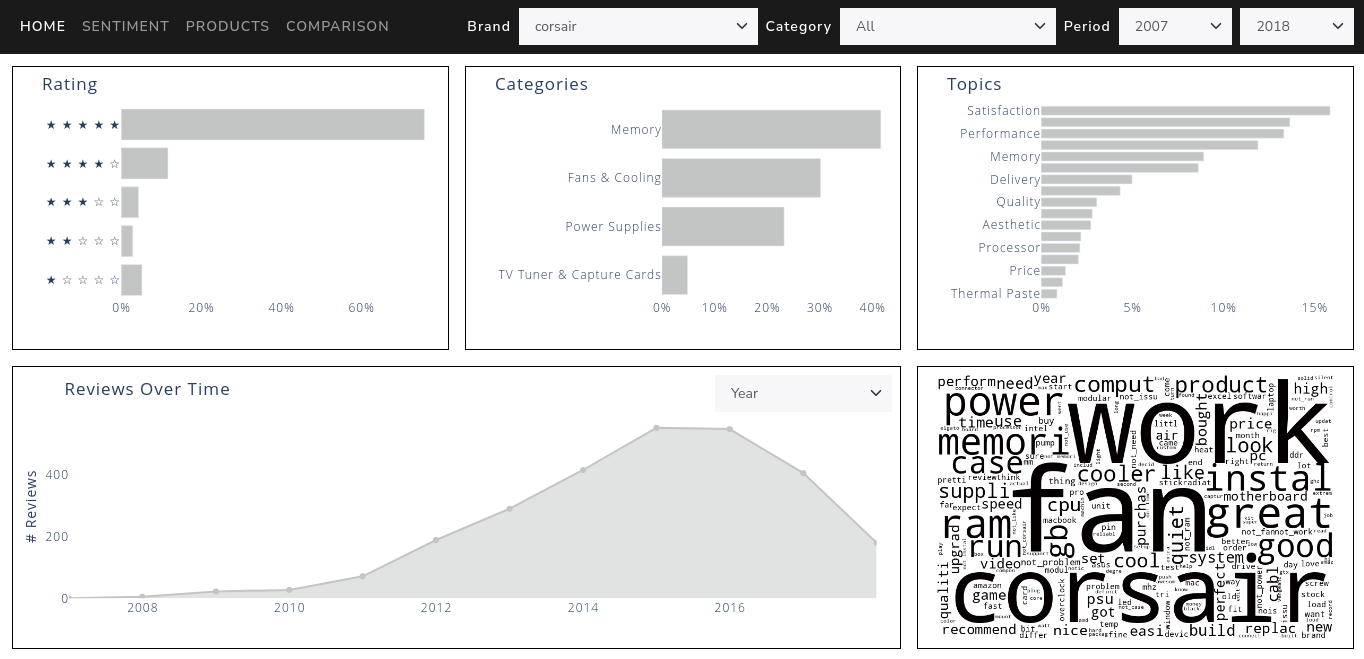
\includegraphics[width=0.95\textwidth]{images/dashboard/dashboard_home.png}
  \caption{Screenshot che mostra la pagina principale della dashboard}
  \label{fig:dashboard1}
\end{figure}

Una pagina specifica dedicata all'analisi del sentiment (figura \ref{fig:dashboard2}) è stata realizzata monitorando il sentiment generale nel tempo per categoria e per i topic.

\begin{figure}[ht]
  \centering
  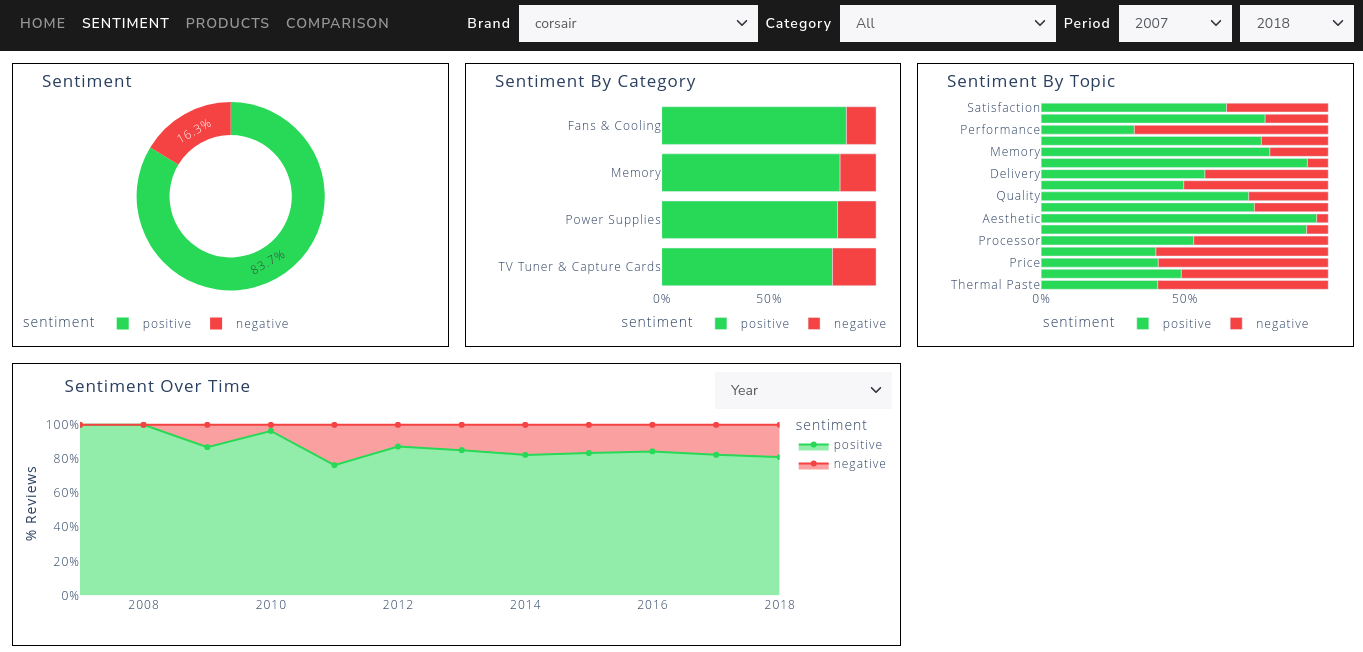
\includegraphics[width=0.95\textwidth]{images/dashboard/dashboard_sentiment.png}
  \caption{Screenshot che mostra la pagina relativa all'analisi del sentiment della dashboard}
  \label{fig:dashboard2}
\end{figure}

\newpage

Un'ulteriore pagina (figura \ref{fig:dashboard3}) permette di mostrare i prodotti di un brand con le relative recensioni e con analisi sul sentiment e i topic.

\begin{figure}[ht]
  \centering
  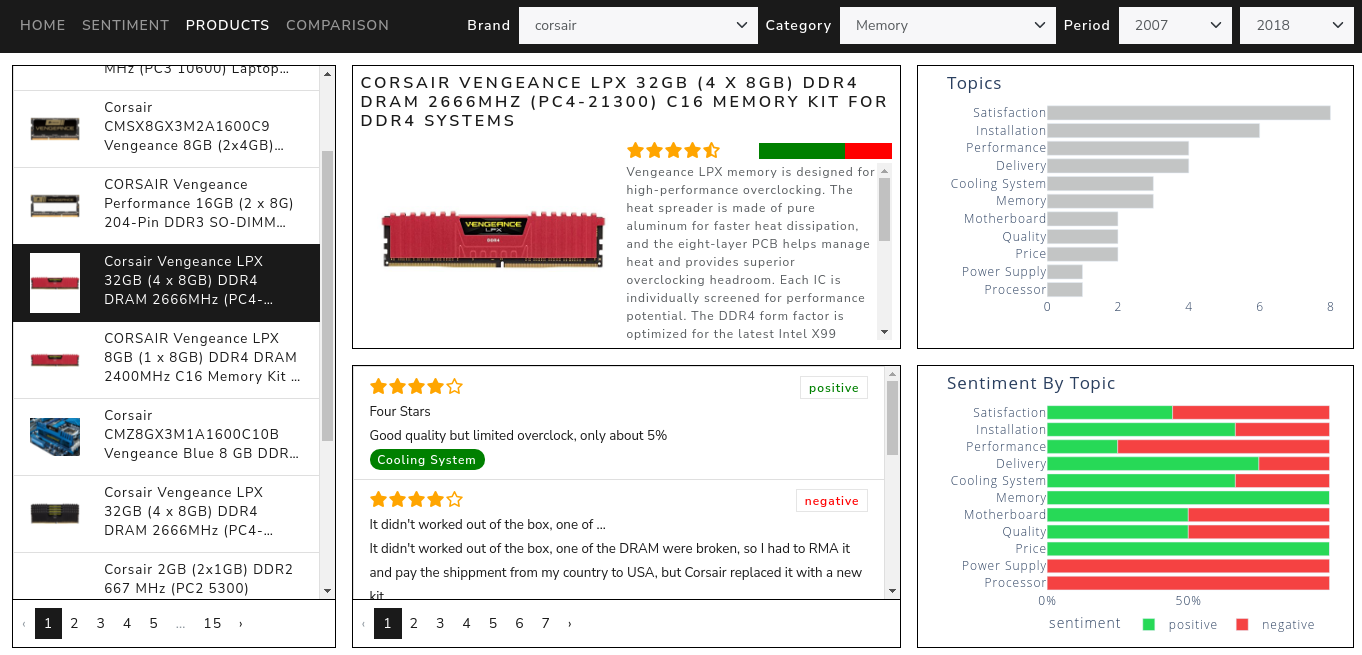
\includegraphics[width=0.95\textwidth]{images/dashboard/dashboard_products.png}
  \caption{Screenshot che mostra la pagina relativa ai prodotti della dashboard}
  \label{fig:dashboard3}
\end{figure}

Infine scelto un brand è possibile compararlo con i competitor più importanti analizzando le differenze nel sentiment nel tempo e gli aspetti (figura \ref{fig:dashboard4}).

\begin{figure}[ht]
  \centering
  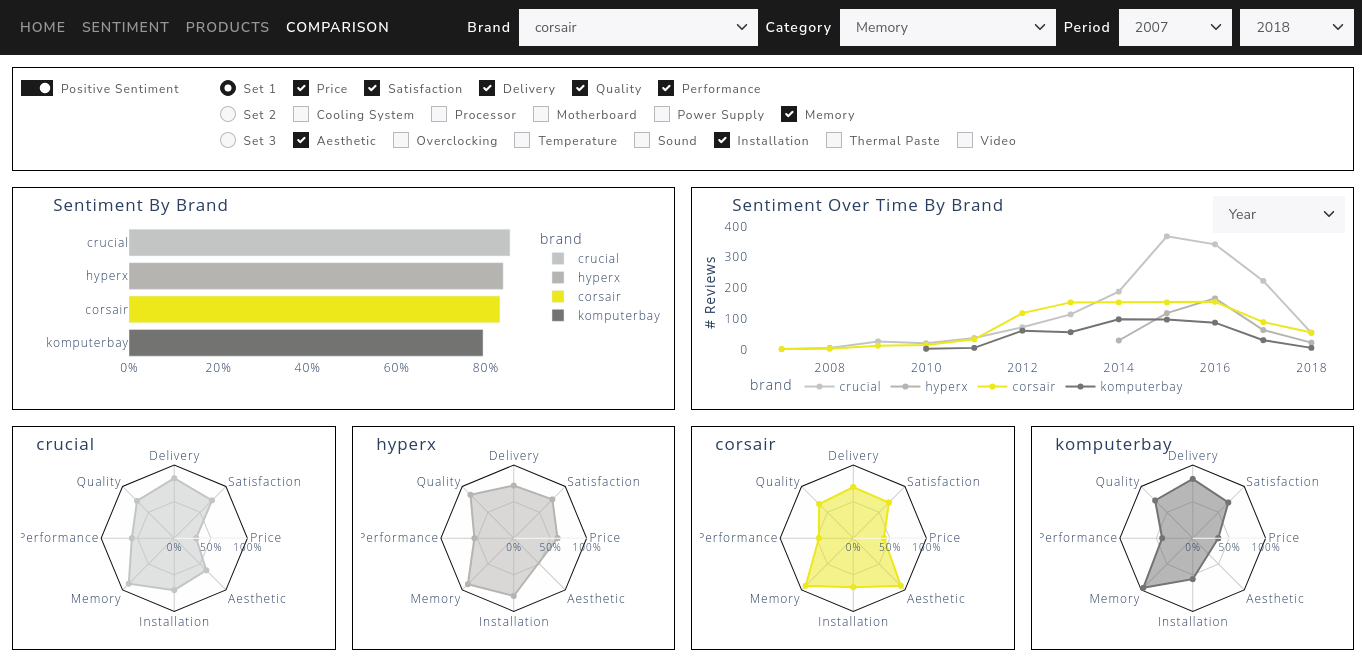
\includegraphics[width=0.95\textwidth]{images/dashboard/dashboard_comparison.png}
  \caption{Screenshot che mostra la pagina relativa ai brand della dashboard}
  \label{fig:dashboard4}
\end{figure}